\documentclass[12pt,a4paper]{article}

\usepackage[margin=1in]{geometry}
\usepackage[T1]{fontenc}
\usepackage[utf8]{inputenc}
\usepackage{lmodern}
\usepackage{setspace}
\usepackage{titlesec}
\usepackage{hyperref}
\usepackage{longtable}
\usepackage{booktabs}
\usepackage{array}
\usepackage{enumitem}
\usepackage{graphicx}
\usepackage{xcolor}
\usepackage{float}
\usepackage{tikz}
\usetikzlibrary{arrows.meta, positioning, fit, backgrounds}

\hypersetup{
	colorlinks=true,
	linkcolor=blue!60!black,
	urlcolor=blue!60!black,
	pdftitle={MoneyMentor AI Project Report},
	pdfauthor={MoneyMentor AI Team}
}

\setstretch{1.15}
\setlist[itemize]{leftmargin=1.5em}
\setlist[enumerate]{leftmargin=1.7em}

\titleformat{\section}{\large\bfseries}{\thesection.}{0.6em}{}
\titleformat{\subsection}{\normalsize\bfseries}{\thesubsection.}{0.5em}{}

\title{\textbf{MoneyMentor AI}\\
Formal Project Report}
\author{ET AI Hackathon 2026 Submission}
\date{March 2026}

\begin{document}

\maketitle
\tableofcontents
\newpage

\section{Abstract}
MoneyMentor AI is a full-stack personal finance platform designed for Indian users, focused on deterministic tax computation, portfolio diagnostics, financial health scoring, retirement planning, affordability checks, budgeting assistance, and proactive policy alerts. The system combines a Python FastAPI backend and a Next.js frontend with modular route-based architecture. It supports both deterministic computation and selective LLM augmentation for parsing and advisory features. This report presents the implemented architecture, technical modules, API surface, data flow, algorithmic logic, operational characteristics, and current limitations.

\section{Problem Statement and Motivation}
Indian salaried users often struggle with fragmented financial decision-making across tax planning, investments, debt management, and long-term planning. Existing solutions are either too narrow (single use case) or advisory-heavy with low transparency.

The project addresses this by delivering:
\begin{itemize}
	\item Deterministic and auditable tax computations for FY 2025--26.
	\item Multi-tool financial workflows in a unified interface.
	\item Document ingestion for Form 16 and CAMS statements.
	\item Actionable guidance in user-readable language.
\end{itemize}

\section{Project Objectives}
Primary objectives are:
\begin{enumerate}
	\item Build a modular finance platform with separate tax, portfolio, health, FIRE, affordability, budget, and alerts tools.
	\item Ensure backend logic is deterministic where financial correctness is critical.
	\item Use AI selectively for extraction and recommendations, not core arithmetic.
	\item Provide a premium multi-page web UX with responsive route-based pages.
	\item Support fast demo mode through precomputed persona responses.
\end{enumerate}

\section{Technology Stack}
\subsection{Backend}
\begin{itemize}
	\item Framework: FastAPI
	\item Runtime: Python 3.x
	\item Validation: Pydantic models
	\item PDF parsing: pdfplumber
	\item AI integration: OpenAI (chat + vision fallback)
\end{itemize}

\subsection{Frontend}
\begin{itemize}
	\item Framework: Next.js 14 (App Router)
	\item UI library: React 18
	\item Styling: Tailwind CSS + custom global design system
	\item Motion: Framer Motion
\end{itemize}

\section{Implemented Repository Structure}
The implemented codebase follows this high-level structure:
\begin{itemize}
	\item \texttt{backend/}: API server, domain schemas, computation engines, services, and routes.
	\item \texttt{frontend/}: Next.js application pages, reusable components, and API client.
	\item \texttt{generate\_mock\_data.py}: utility script generating synthetic Form 16 and CAMS PDFs.
	\item \texttt{mock\_data/}: generated test statements used in upload flows.
	\item Documentation files: \texttt{README.md}, \texttt{walkthrough.md}, \texttt{implementation\_plan.md}.
\end{itemize}

\section{System Architecture}
\subsection{Logical Architecture Diagram}
\begin{figure}[H]
\centering
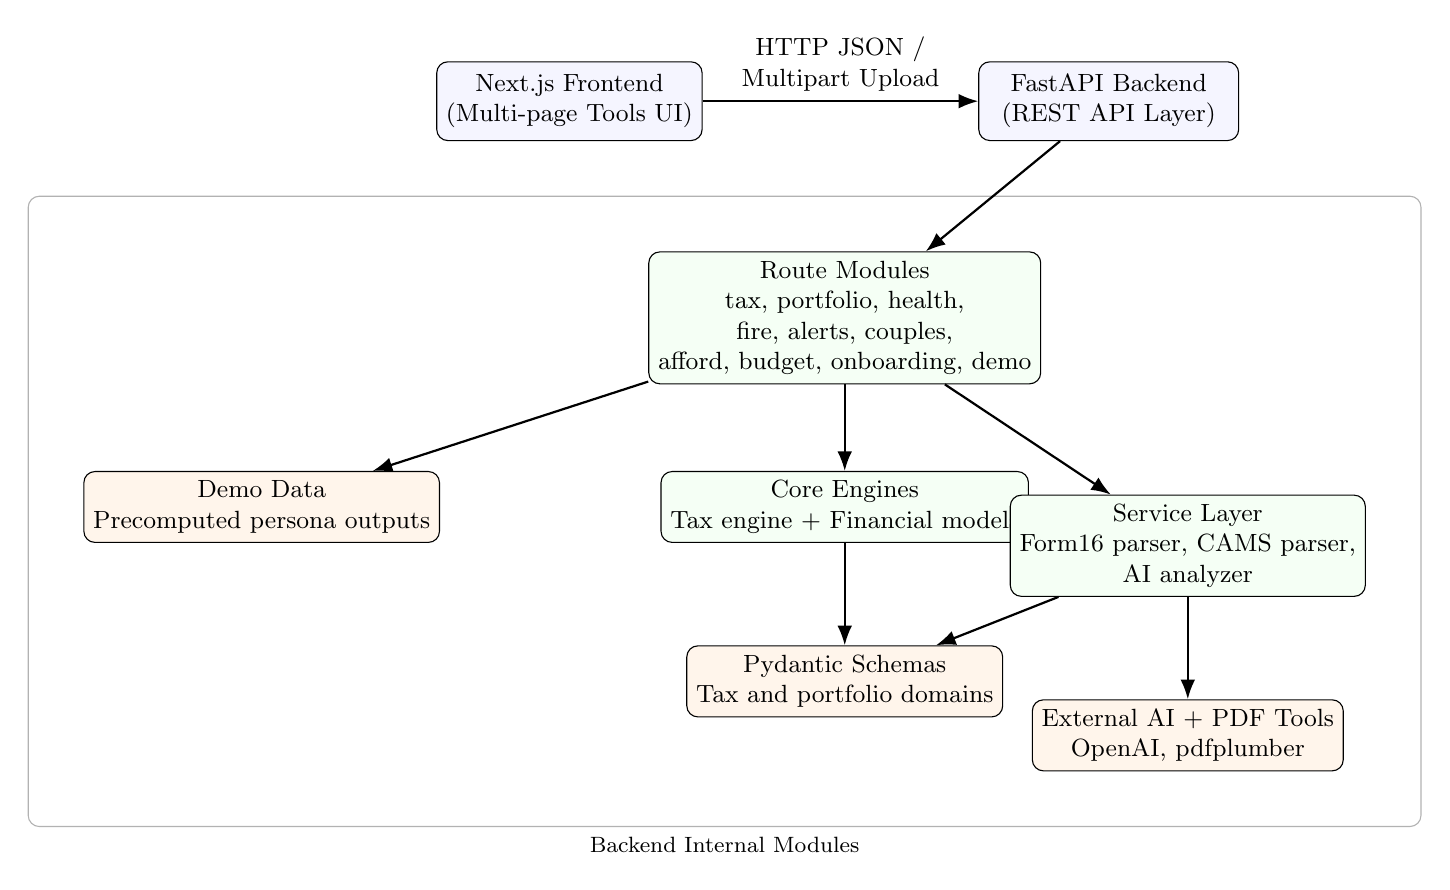
\begin{tikzpicture}[
	font=\small,
	node distance=10mm and 14mm,
	box/.style={draw, rounded corners, align=center, minimum width=33mm, minimum height=10mm, fill=blue!4},
	svc/.style={draw, rounded corners, align=center, minimum width=30mm, minimum height=9mm, fill=green!4},
	data/.style={draw, rounded corners, align=center, minimum width=28mm, minimum height=9mm, fill=orange!8},
	arr/.style={-{Latex[length=2.5mm]}, thick}
]

\node[box] (ui) {Next.js Frontend\\(Multi-page Tools UI)};
\node[box, right=35mm of ui] (api) {FastAPI Backend\\(REST API Layer)};

\node[svc, below left=14mm and -8mm of api] (routes) {Route Modules\\tax, portfolio, health,\\fire, alerts, couples,\\afford, budget, onboarding, demo};
\node[svc, below=11mm of routes] (core) {Core Engines\\Tax engine + Financial models};
\node[svc, below right=14mm and -4mm of routes] (services) {Service Layer\\Form16 parser, CAMS parser,\\AI analyzer};

\node[data, below=13mm of core] (schemas) {Pydantic Schemas\\Tax and portfolio domains};
\node[data, below=13mm of services] (ext) {External AI + PDF Tools\\OpenAI, pdfplumber};
\node[data, left=28mm of core] (demo) {Demo Data\\Precomputed persona outputs};

\draw[arr] (ui) -- node[above, align=center]{HTTP JSON /\\Multipart Upload} (api);
\draw[arr] (api) -- (routes);
\draw[arr] (routes) -- (core);
\draw[arr] (routes) -- (services);
\draw[arr] (core) -- (schemas);
\draw[arr] (services) -- (schemas);
\draw[arr] (services) -- (ext);
\draw[arr] (routes) -- (demo);

\begin{scope}[on background layer]
	\node[draw=black!30, rounded corners, fit=(routes)(core)(services)(schemas)(ext)(demo), inner sep=7mm, label=below:{\footnotesize Backend Internal Modules}] {};
\end{scope}

\end{tikzpicture}
\caption{Implemented architecture of MoneyMentor AI}
\end{figure}

\subsection{Architectural Notes}
\begin{itemize}
	\item The frontend consumes backend APIs through a centralized client in \texttt{frontend/lib/api.js}.
	\item FastAPI acts as the orchestration layer and delegates to route handlers.
	\item Deterministic math is isolated in \texttt{core/tax\_engine.py} and \texttt{core/financial\_models.py}.
	\item Parsing and LLM-dependent work is isolated in \texttt{services/} to preserve separation of concerns.
\end{itemize}

\section{Backend Design}
\subsection{Application Bootstrap}
The backend entry point initializes FastAPI with CORS configuration and includes modular routers. A global exception handler standardizes failure responses. Health and root endpoints provide service discoverability.

\subsection{Configuration Layer}
\texttt{config/settings.py} centralizes environment-driven settings such as API keys, model names, frontend origin, and upload constraints.

\subsection{Domain Models}
Two schema modules are used:
\begin{itemize}
	\item \texttt{core/schemas.py}: tax domain models (salary, deductions, regime comparison, analysis output).
	\item \texttt{core/portfolio\_schemas.py}: portfolio, health, FIRE, and alerts models.
\end{itemize}

\subsection{Core Engines}
\subsubsection{Tax Engine}
The tax engine implements:
\begin{itemize}
	\item Old and New regime slab computations.
	\item Standard deduction differences.
	\item Section 87A rebate logic.
	\item Surcharge and cess handling.
	\item HRA exemption and deduction utilization checks.
	\item Missed deduction identification with estimated potential savings.
\end{itemize}

\subsubsection{Financial Models}
Financial models include:
\begin{itemize}
	\item XIRR and CAGR approximations.
	\item Fund overlap estimation and alert generation.
	\item Expense ratio drag quantification.
	\item Benchmark comparison against NIFTY50 reference return.
	\item Rebalancing recommendations by category target.
	\item Health scoring primitives (emergency fund, insurance, debt, tax efficiency, retirement readiness).
	\item FIRE projection engine with inflation-adjusted corpus targets.
\end{itemize}

\subsection{Service Layer}
\subsubsection{Form 16 Parsing Pipeline}
The parser executes a four-step strategy:
\begin{enumerate}
	\item PDF text and table extraction via pdfplumber.
	\item Regex extraction for known field patterns.
	\item GPT text extraction fallback for weakly structured content.
	\item GPT vision fallback for image-like scans.
\end{enumerate}

\subsubsection{CAMS Parsing Pipeline}
CAMS extraction follows a similar staged pattern:
\begin{enumerate}
	\item Text extraction.
	\item Regex and line-based parser.
	\item GPT text fallback.
	\item GPT vision fallback.
\end{enumerate}

\subsubsection{AI Analyzer}
Advisory generation functions produce action plans, summaries, and onboarding routing. Deterministic fallback behavior exists for unavailable model output.

\subsection{API Modules}
Implemented routes are grouped by financial function:
\begin{itemize}
	\item Tax: upload, analyze, quick analyze.
	\item Portfolio: CAMS upload and analysis.
	\item Health score calculation.
	\item FIRE planning.
	\item Proactive alerts.
	\item Couples planning.
	\item Affordability advisor.
	\item Budget planner.
	\item Onboarding recommendation.
	\item Demo persona endpoints.
\end{itemize}

\section{Frontend Design}
\subsection{Routing and Page Composition}
The frontend uses Next.js App Router. Each feature has its own route segment and generally wraps content with a shared sub-layout containing header and footer. Dedicated pages exist for:
\begin{itemize}
	\item Landing page and onboarding flow.
	\item Tax workflow and dashboard.
	\item Portfolio, health, FIRE, afford, budget, couples, alerts.
	\item ET article style integration page.
\end{itemize}

\subsection{Component System}
Reusable components include navigation, upload interactions, summary widgets, deductions/action cards, and demo persona loader. The visual system is centralized in \texttt{app/globals.css} with dark/light variables and typography tokens.

\subsection{Client API Abstraction}
\texttt{frontend/lib/api.js} exposes typed helper functions that map to backend endpoints and centralize error handling for GET/POST and multipart upload operations.

\section{End-to-End Data Flows}
\subsection{Tax Analysis Flow}
\begin{enumerate}
	\item User uploads Form 16 PDF on the tax page.
	\item Backend parser extracts structured tax profile.
	\item Analysis endpoint computes old/new tax and missed deductions.
	\item AI advisory generation produces action plan and summary.
	\item Frontend dashboard renders comparison and recommendations.
\end{enumerate}

\subsection{Portfolio Flow}
\begin{enumerate}
	\item User uploads CAMS statement.
	\item Parser extracts holdings.
	\item Analysis computes returns, overlap, expense drag, and rebalancing.
	\item Frontend renders holdings table and strategy insights.
\end{enumerate}

\subsection{Health and FIRE Flow}
User-provided structured inputs are sent to dedicated endpoints that run deterministic scoring/projection logic and return metrics plus action guidance.

\section{Security and Privacy Characteristics}
Observed privacy posture from implementation:
\begin{itemize}
	\item Upload processing is designed for transient analysis without database persistence.
	\item Frontend communicates directly with backend over controlled origin settings.
	\item Input validation exists for file type and file size constraints.
	\item Environment variables are externalized via settings and \texttt{.env} pattern.
\end{itemize}

\section{API Surface Summary}
\begin{longtable}{p{0.18\linewidth} p{0.34\linewidth} p{0.43\linewidth}}
\toprule
\textbf{Method} & \textbf{Endpoint} & \textbf{Purpose} \\
\midrule
POST & /api/upload-form16 & Parse Form 16 PDF to tax profile \\
POST & /api/analyze-tax & Full tax analysis with recommendations \\
POST & /api/quick-analyze & Deterministic tax-only quick analysis \\
POST & /api/upload-cams & Parse CAMS/KFintech statement \\
POST & /api/analyze-portfolio & Portfolio diagnostics and recommendations \\
POST & /api/health-score & Six-dimensional health score generation \\
POST & /api/fire-plan & FIRE projection and milestone plan \\
GET & /api/alerts & Personalized policy and market alerts \\
POST & /api/couples-plan & Joint optimization for couples \\
POST & /api/affordability-check & Purchase affordability verdict \\
POST & /api/budget-plan & AI-assisted budget optimization \\
POST & /api/onboarding & Questionnaire-driven tool routing \\
GET & /api/demo/* & Persona-based demo payloads \\
GET & /api/health & Service health endpoint \\
\bottomrule
\end{longtable}

\section{Testing and Verification Strategy}
The current repository includes manual and demo-driven verification artifacts. A robust test strategy should include:
\begin{enumerate}
	\item Unit tests for slab tax, rebate boundaries, surcharge transitions, and deduction limits.
	\item Property tests for parser robustness across noisy PDF text.
	\item Contract tests between frontend client and backend schema outputs.
	\item End-to-end UI automation for critical flows (tax upload, portfolio upload, onboarding route).
	\item Performance testing under concurrent uploads.
\end{enumerate}

\section{Strengths, Risks, and Limitations}
\subsection{Strengths}
\begin{itemize}
	\item Clear separation of concerns across routes, services, and core engines.
	\item Strong deterministic computation base for financial correctness.
	\item Broad functional coverage in one integrated product.
	\item Effective fallback strategy for difficult document parsing.
\end{itemize}

\subsection{Current Risks and Limitations}
\begin{itemize}
	\item LLM extraction quality remains document-quality dependent.
	\item No persistent datastore means no historical trend analytics yet.
	\item Some calculation paths use approximations (for example, simplified CAGR assumptions in portfolio flow).
	\item Formal automated test suite is not yet fully integrated in the visible repository.
\end{itemize}

\section{Future Work}
Priority enhancements:
\begin{enumerate}
	\item Add persistent user profile and encrypted report history.
	\item Improve parser confidence scoring and human-readable extraction trace.
	\item Integrate exact transaction-date XIRR with richer statement parsing.
	\item Introduce role-based auth, audit logging, and production observability.
	\item Build CI pipelines for linting, tests, and schema contract checks.
\end{enumerate}

\section{Conclusion}
MoneyMentor AI is implemented as a modular full-stack financial assistant with deterministic tax and financial engines at its core and selective AI augmentation for extraction and recommendations. The architecture is coherent, extensible, and suitable for hackathon demonstration while still aligned with production-minded decomposition. With stronger automated validation, persistence, and operational hardening, the current foundation can evolve into a scalable financial decision platform.

\vspace{1em}
\noindent\textbf{End of Report}

\end{document}
